%!TEX root = ../dissertation.tex
\Chapter{Conclusion}
\label{conclusion}

\newthought{We have become acquainted} with a general framework for modeling cognition as a sequential decision problem: metalevel Markov decision processes. We saw how the framework can be applied to derive rational mechanistic models in three different domains: attention, memory, and planning. And in each case, we found that human behavior showed substantial qualitative alignment with the optimal metalevel policy. Taken together, the results suggest that human cognitive processes are well-adapted to the internal environments in which they operate. More importantly, by formally characterizing the problems posed by those mental environments, and their optimal solutions, we have developed a richer understanding of human cognition in each of these domains.

The breadth of domains covered in Chapters~3-5 is substantial, but the models share many core features. Although Chapters~\ref{sec:attention} and~\ref{sec:memory} considered very different tasks (attention in choice and memory recall), they relied on essentially the same state space and transition structure, based on Gaussian evidence accumulation. This parallels the breadth of domains in which evidence accumulation models have been applied. Our model of planning (Chapter~\ref{sec:planning}) employed a very different type of state space (decision trees), but it shares with Chapter~\ref{sec:attention} the idea that decision-making can be understood as gathering information about rewards (c.f. \citealp{tajima2016optimal,sezener2019optimizing}). All three chapters rely on probabilistic models that specify how the effects of computations relate to an unknown world state. Although these similarities may undercut the claimed generality of the approach, they can also be viewed as a strength. By specifying models using a common framework, it is easier to transfer concepts and computational tools between domains.

\section{Kindred efforts}\label{sec:kindred}

The idea of modeling cognitive processes as optimal solutions to sequential decision problems is not unique to this dissertation. There are at least three major strands of research in this area. I briefly review these strands below, noting similarities and differences to our approach.

\subsection{Optimal evidence accumulation}

As mentioned in the introduction, there is a long history of modeling optimal speed-accuracy tradeoffs using evidence accumulation models. Early work (e.g., \citealp{bogacz2006physics,vul2009one}) focused on binary choices with accuracy-based rewards (e.g., +1 for correct responses) and known evidence coherence (i.e., the strength of evidence supporting the correct response is always the same). In these cases, the optimal stopping rule is given \emph{sequential probability ratio test} (SPRT): continue collecting evidence until a threshold level of evidence is reached either for or against the hypothesis. However, when any of these assumptions are violated, the SPRT (and by extension) is no longer optimal.

By explicitly modeling evidence accumulation as a sequential decision problem, \citet{drugowitsch2012cost} were able to derive the optimal stopping rule when evidence coherence varies from trial to trial.\footnote{%
  This problem is more complex because one cannot simply sum up the log likelihoods for each piece of evidence (which could support option A or B). One must maintain a full belief state over the drift rate, which specifies both the correct answer and the coherence (higher absolute values correspond to higher coherence). 
} This model adopts the same basic evidence accumulation and belief updating dynamics as we used in Chapter~\ref{sec:attention} and~\ref{sec:memory}, with a single accumulator tracking relative evidence for one choice vs. the other. They showed that the optimal policy corresponds to a threshold that changes over time (rapidly expanding and then slowly collapsing). Building on this work, \citet{tajima2016optimal} characterized the optimal decision thresholds for value-based choices, where both importance and difficulty depend on the difference in value between the choice options (c.f. \citealp{fudenberg2018speed}). Going further, \citet{tajima2019optimal} characterizes the optimal solution for three-alternative choices, where the mental states and thresholds reside in an three-dimensional space (including time).

Despite this richness, all the models mentioned above assume a very simple cognitive architecture, in which there are only two possible cognitive operations: gather more evidence, or stop. Building on the Tajima et al. model, \citet{jang2021optimal} derived the optimal policy for the case when the agent can only sample from one item at a time (more precisely, when the value of the attended item produces less noisy samples). Without switching costs, \citet{fudenberg2018speed} showed that it is optimal to perfectly balance attention to each item (alternating at each time step), but in the presence of switching costs, the optimal policy takes on a more interesting structure. As we showed in Chapter~\ref{sec:attention}, the optimal policy takes on even richer structure when there are more than two alternatives, preferentially attending to items with high estimated value. However, the high dimensionality of the state space makes it impossible to exactly identify the optimal policy for trinary choice using backwards induction (the method employed in the Drugowitsch, Tajima, and Jang papers; described in Section~\ref{sec:backinduct}). We were only able to (approximately) identify the optimal policy in this case using the BMPS algorithm (Section~\ref{sec:bmps}), which we developed specifically to solve metalevel MDPs. This highlights the value of using a formalism that is tailored to the specific type of sequential decision problems posed by cognition.

Another line of work in economics has also sought to characterize optimal evidence accumulation in cases where the agent can control the nature of evidence sampled \citep{woodford2014stochastic,hebert2017rational}. The key distinguishing feature of these models is the assumption of a very flexible cognitive architecture in which the agent can gather an arbitrary form evidence at each time step (formally a conditional distribution of a signal given the true world state). Paradoxically, allowing for such flexibility actually makes it easier\footnote{%
  Assuming you have the math training of an Econ PhD.
} to identify the optimal policy, as it can be derived analytically. However, this flexibility may limit the ability of these models to account for human cognitive processes, which are likely adapted to more restrictive architectures.

\subsection{POMDP models of visual search}

Another area where optimal sequential models are often found is in visual search. In these tasks, participants are asked to find a target object hidden among distractors in an image. Early work in this area suggested that people fixate on areas where the target is most likely to be \citep{najemnik2005optimal}. This strategy can be understood as a myopic policy (in precisely the sense of Section~\ref{sec:myopic}) for a metalevel MDP, as it maximizes the chance of identifying the target on the very next time step. However, as we have seen, myopic policies are often suboptimal. Recognizing this, \citet{butko2008ipomdp} reformulated the ``ideal observer'' model of Najemnik and Geisler as an ``information-gathering POMDP'', a special case of POMDPs in which the state does not change and actions serve only to generate information. This is exactly the same restriction made by metalevel MDPs (see Section~\ref{sec:pomdp}). However, rather than using a reward function capturing the cost of fixations and the reward for finding the target (as we would do in the metalevel MDP approach), they assumed a reward function that directly rewards reduction of entropy in the belief state. Nevertheless, they found that the learned policy found the target faster than the ideal observer model.

Taking an approach more similar to ours, \citet{acharya2017human} present a POMDP model in which the reward exactly captures the incentives of the task and the opportunity cost of time. Indeed, this model can be viewed as a metalevel MDP in which fixations correspond to computations (as in Chapter~\ref{sec:attention}). Applying the model to the distractor-ratio task, they found that the optimal fixation policy better captured qualitative patterns in human fixation data compared to the ideal observer model. In parallel, \citet{hoppe2019multistep} conducted an experiment specifically designed to distinguish myopic and planned eye movements (this involved using oddly shaped search regions and allowing participants to make exactly one or two fixations). They model the task as an MDP and find that the optimal policy predicts people's average fixation locations almost shockingly well, predicting exactly when and how people deviate from the myopic ideal observer model.

\subsection{POMDP models of decision-making}\label{sec:alternative-pomdp}

Most similar to our work, researchers have recently begun to use POMDPs to model decision-making processes. Building on the models of visual search described above, \citet{chen2017cognitive} present a model of how people direct their eye fixations when making a decision based on information presented in a table. They find that both people and the optimal policy use decision strategies that collect intermediate amounts of information compared to classical strategies (such as take-the-best \citealp{gigerenzer1996reasoning}). This parallels our own predictions and findings in a metalevel MDP model of multi-attribute choice \citep{gul2018discovering}.

In all the POMDP models mentioned so far, the ``computations'' correspond to gathering information from an external environment. To some extent, this can also be said of the models in this dissertation (although, in Chapters~\ref{sec:attention} and~\ref{sec:memory}, there is good reason to believe that people's fixations are more indicative of internal processing than true information gathering). In very exciting new work, \citet{chen2021apparently} present a POMDP model of risky choice in which the actions correspond to truly internal operations such as making ordinal comparisons of payoff probabilities and computing a noisy estimate of expected value. They find that, when the expected value computation is very noisy, the optimal policy relies more on the more robust comparison operations. This improves performance, but yields systematic choice biases (decoy effects). Although all of the work reviewed so far takes a fully Bayesian view of computation (making no distinction between mental states and belief states), \citet{oulasvirta2022computational} propose a general POMDP framework in which an agent interacts with an ``internal environment'' which is defined by ``mental states'', suggesting that the framework could be applied more generally (although I am not aware of any concrete examples of this more general case).

In light of all the work reviewed in this section, we might ask again: why bother with metalevel MDPs? The answer, I think, comes down to what level of generality we would like to have in a framework for developing optimal sequential models of cognition. Models of evidence accumulation are typically posed in very specific terms, directly specifying the dynamic programming problem for a given decision-making task. On the other end, the POMDP models are posed in very general terms, as just one instance of the problem of interacting with a dynamic and partially observable environment. Metalevel MDPs taken an intermediate approach. They are general enough to model many different types of cognitive processes within one framework, but they are specific enough to \emph{only} model cognitive processes (or more generally, computational processes). In particular, metalevel MDPs formally distinguish between internal and external states and actions. Although this can be limiting (as discussed below), it has important conceptual and technical benefits. Emphasizing the latter, the POMDP models of decision-making discussed above use artificially simplified state spaces, for example, treating continuous features as binary \citep{chen2017cognitive}, or assuming a small number of operations per episode \citep{chen2021apparently}). This is likely because the general-purpose reinforcement learning approaches they employ would not have performed well in larger state spaces. Using metalevel MDPs, we were able to identify optimal policies in richer cognitive architectures than would be feasible when treating the problem as a generic POMDP.

\section{Points of weakness and avenues for growth}

There are several dimensions on which the framework could be extended in future work.

\subsection{Learning the metalevel homunculus}\label{sec:homunculus}

One of the most significant challenges for the metalevel MDP framework is the problem of infinite regress. As mentioned in the Introduction (Section~\ref{sec:bound-meta}), the framework assumes that people are \emph{metalevel rational}, meaning that they choose computational actions to optimally balance a cost-benefit tradeoff. However, it does not explain how those choices are themselves made. In this way, the framework assumes a ``metalevel homunculus'': an unbounded, perfectly rational agent that always knows just what thought to think next (c.f. \citealp{hazy2006banishing,botvinick2014computational}). Explaining (or perhaps explaining away) the homunculus is critical for these models to provide a complete explanation of how people effectively allocate computational resources.

Perhaps the most plausible theory of the metalevel homunculus is that it is learned. Indeed, learning has been a critical aspect of many models of metalevel control in psychology. The earliest examples are found in cognitive architectures like ACT-R and SOAR, which have simple mechanisms for learning when to apply different production rules \citep{laird1986chunking}. However, like early models of strategy selection \citep{shrager1998scads}, this type of learning was primarily associative. The idea that a metalevel controller explicitly learns to maximize reward was proposed in later strategy selection models \citep{erev2005adaptation,rieskamp2006ssl,lieder2017strategy}. Building on this work, \citep{lieder2018rational} developed the Learned Value of Control (LVOC) model, which learns metalevel policies at the level of individual cognitive operations; this model has since been applied to the Mouselab-MDP task developed in Chapter~\ref{sec:planning} \citep{jain2019how}. Reinforcement learning (RL) has also been proposed as the mechanism by which people learn which goals to pursue \citep{cushman2015habitual}, and when to retrieve and store information in working memory \citep{oreilly2006making,todd2008learning} and episodic memory \citep{lu2022neural}. 

Metalevel MDPs provide a natural framework in which to cast theories of metacognitive RL. However, explicitly formalizing the metalevel control problem in this way also reveals a major challenge: learning good policies in metalevel MDPs is ``exceptionally difficult'' \citep{hay2016principles}. For example, my colleagues and I have shown that a widely used deep reinforcement learning method (a DQN; \citealp{mnih2015humanlevel}) is unable to learn a good policy in a simplified form of the attention metalevel MDP from Chapter~\ref{sec:attention} \citep{callaway2018learning}. In a more complex problem (the game of Hex), \citet{hay2016principles} showed that a learned metalevel policy can outperform a standard Monte Carlo tree search algorithm \citep{kocsis2006bandit}, but only when the number of iterations is very limited (20 or less). Why is it so challenging to learn policies for metalevel MDPs? There are at least three reasons: metalevel MDPs are characterized by (1) large state spaces, (2) stochastic dynamics, and (3) sparse rewards. Reward sparsity is perhaps the most challenging, as it induces an extreme temporal credit assignment problem. In each episode, the agent takes many computations, but receives only a single external reward. It is thus not clear which computations should receive ``credit'' for large rewards. 

One way to make learning easier in the presence of sparse rewards is to adjust the reward function by adding \emph{shaping rewards} (or ``pseudo rewards'') that provide more immediate feedback about the value of each (mental) action that is executed \citep{ng1999policy}. For example, shaping rewards derived from the optimal metalevel value functions can accelerate human learning in the Mouselab MDP task used in Chapter~\ref{sec:planning} \citep{callaway2022leveraging}. Although people would not have access to such perfect shaping rewards in the real world, they may have access to simpler but still useful surrogates.\footnote{%
  \citet{hay2016principles} propose one intuitively appealing shaping reward based on the difference in the expected value of taking an external action in the mental states before and after executing a computation. However, the results were, in his terms, ``not yet as good as we'd like''.
} That is, people may experience a reward when they have a ``good thought'' even if it does not immediately lead to an external action \citep{gopnik1998explanation}. Indeed, people appear to place value on external information that cannot be acted on \citep{eliaz2007experimental,gottlieb2018neuroscience}, and researchers have begun to formalize the specific qualities of information that people value \citep{markant2014preference,markant2016selfdirected}. This suggests a fascinating research question: what factors elicit the subjective experience of having a good thought?


\subsection{Partially observable minds}\label{sec:partially-observable}

% A key assumption of the metalevel DMP framework is that the agent has direct access to the mental state. Indeed, 

A key structural assumption in the framework is the distinction between the mental state and the world state. The defining features of the mental state are that it can be affected by computation, and that it is directly accessible to the agent. However, these two features do not need to coincide. It is possible that we do not have complete access to aspects of our mental state that we can nevertheless control to some extent. This possibility was suggested by \citet{suchow2016deciding}, who proposed a POMDP model of working memory maintenance. In this model, the agent selects mental actions to increase the activation level of a selected memory, but the current activation levels can only be imperfectly measured.

To allow for partial observability in a metalevel MDP, we can simply assume that the agent does not have direct access to the mental state, but instead has access to an incomplete observation of that state. An interesting question arises as to how these observations should be used. From a POMDP perspective, the observations should be integrated over time into a metalevel belief state (a distribution over mental states). However, this complicates the metalevel controller considerably, creating technical challenges in finding optimal solutions, and exacerbating the homunculus problem described above. An alternative approach, employed by \citet{suchow2016deciding}, is to assume that the metalevel decisions are made based only on the current observation. This yields a simpler and perhaps more psychologically plausible model. However, because observations are not Markovian, one can no longer use standard dynamic programming techniques to find the optimal policy. This further motivates the development of model-free strategies for learning metalevel policies.

\begin{figure*}
  \centering
  \includegraphics[width=0.8\textwidth,page=3,trim=0 50 0 50]{diagrams/metamdp.pdf}
  % 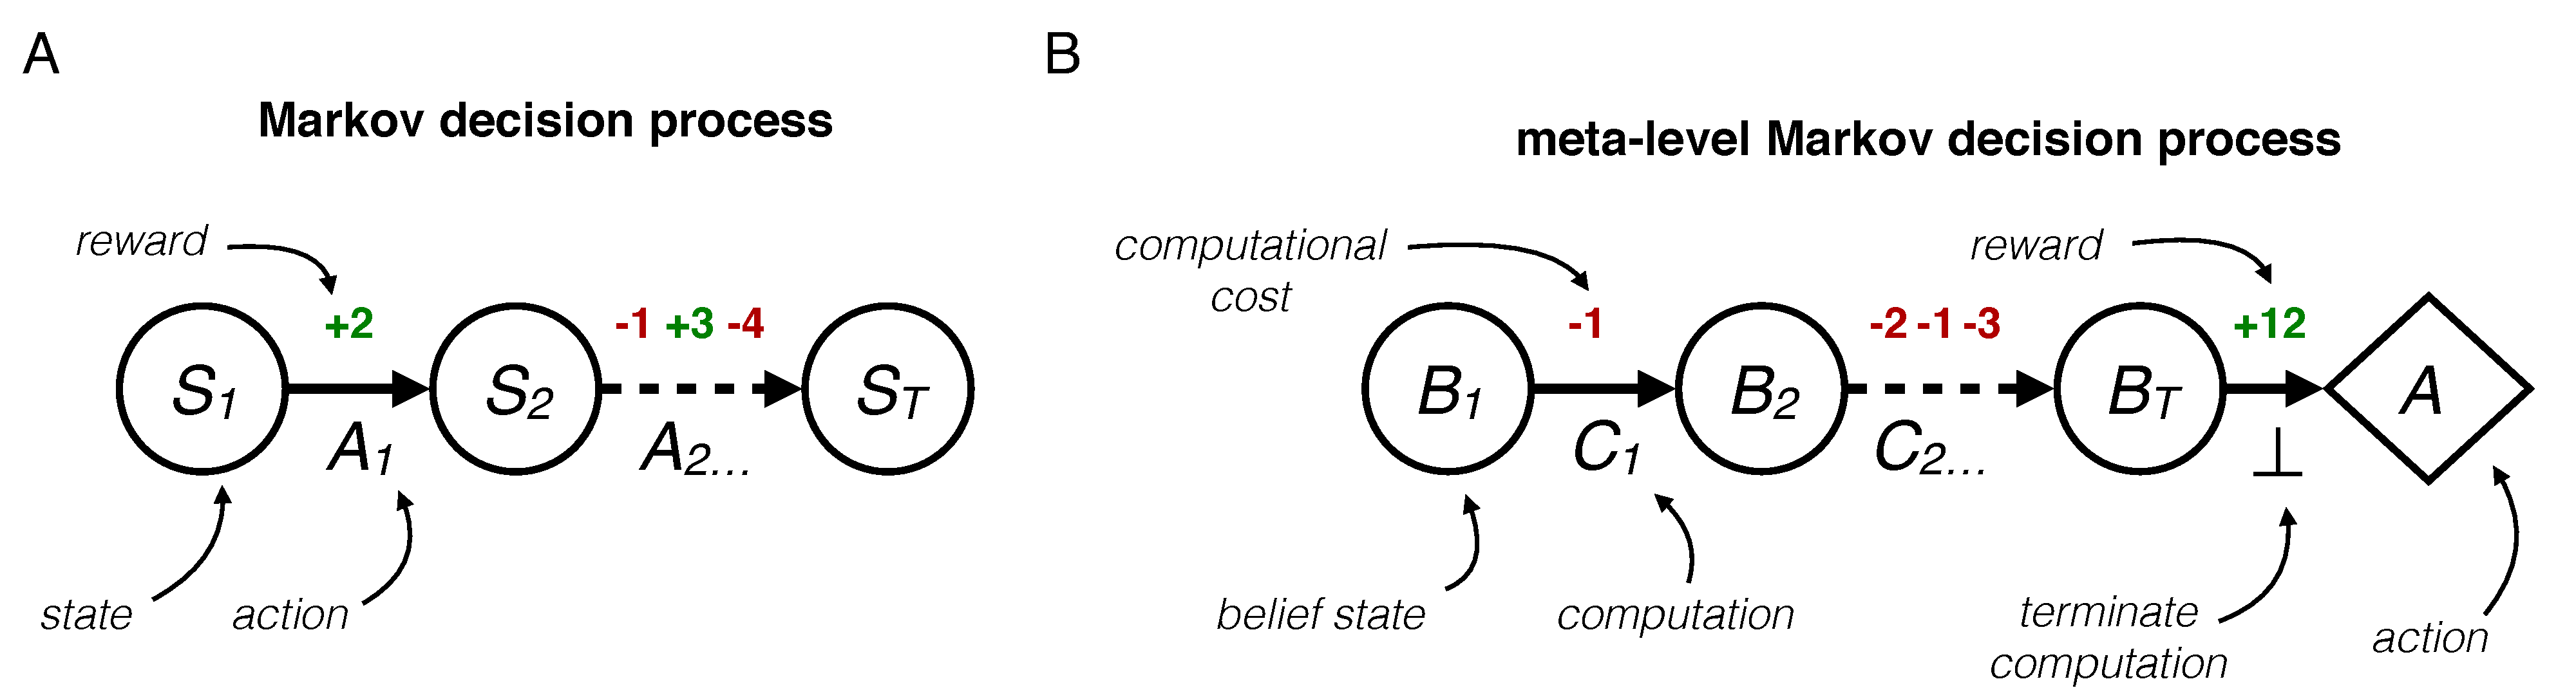
\includegraphics[width=\textwidth]{figs/metamdp.pdf}
  \caption{\captiontitle{Interleaved metalevel MDP}. To formalize the problem of interleaved computation and action, we can augment the metalevel MDP framework to include sequences of world states, actions, and external rewards. Note that there is no cognitive cost in this formalism, as any opportunity costs should be captured in the external reward function. The elements that capture the external environment are indicated in blue.
  }
  \label{fig:metamdp-joint}
\end{figure*}

\subsection{Interleaved computation and action}\label{sec:interleaved}

A second key structural assumption in the framework is that each metalevel episode occurs within a single external timestep. That is, the world state does not change, and only one external action is executed (at the end of the episode). This has two implications. First, it assumes that the agent can think as long as they want without having to worry about the world state changing. Second, it assumes that information considered while choosing one action cannot influence the selection of future actions. Although these assumptions hold approximately in many experimental and naturalistic tasks, they will not hold in fast-paced dynamic problems (e.g. jay walking) or in sequential problems with stochastic dynamics (e.g. chess).

To model interleaved computation and action, we essentially replace the single world state and action with a full external MDP that progresses in lockstep with the metalevel MDP (c.f. joint-state MDPs; \citealp{russell1991right,parr1998reinforcement,hay2016principles}). Figure~\ref{fig:metamdp-joint} illustrates one way this could work. At each timestep the agent selects both a computation and an action (the action may be to simply sit still while thinking). The next world state and reward depend on the current state and action, as in a standard MDP. As in standard metalevel MDPs, the next mental state depends on the current mental state and the computation executed; but it additionally depends on the previous action and the \emph{new} world state. The former captures the fact that the agent may understand how their actions affect the world. The latter captures the agent's ability to perceive the changing world state.

In the interleaved case, the decision about how much to think becomes more nuanced. Specifically, one must not only decide \emph{how much} to think but also \emph{when} to think. In some cases, it may make sense to do all of one's thinking up front, as the standard metalevel MDP assumes. This strategy makes sense because it ensures that every action you take is informed by all the computation you do. However, there are at least three reasons one might want to begin acting before having a complete plan. First, one may be able to continue thinking while executing the early part of the plan, for example considering which way one will turn while walking down a long corridor \citep{oceallaigh2015metareasoning}. Second, if the world dynamics are stochastic, knowing how those transitions unfold will allow the agent to focus their planning on the the situations they actually encounter. Third, forming a complete plan may impose representational costs that could be avoided by only constructing a concrete plan for the immediate future, perhaps having a more abstract plan for the more distant future \citep{ho2020efficiency}.


\subsection{Optimizing the architecture}\label{sec:optimize-architecture}

A third assumption of the framework is that only the policy, and not the metalevel MDP itself, is optimized. This assumption is almost always made in standard applications of MDPs, as the MDP represents the external environment, which the agent has no direct control over. In contrast, because a metalevel MDP represents an agent's internal computational environment, it is likely that the metalevel MDP itself is adapted to the structure of the external problems the agent has to solve.

There are two timescales at which adaptation of an organism's cognitive architecture could occur (in animals): evolutionary and developmental. Clearly, evolution has a major role in shaping the total amount of biological resources allocated to cognition (e.g., brain volume), as well as the ease with which certain types of computations can be learned and executed. However, at the level of abstraction that we have posed metalevel MDPs, the developmental timescale is likely to be more relevant. Indeed, it is natural to view many types of learning as a process of developing new possible mental states and computational actions. For example, as a consequence of reading this dissertation, you have (hopefully) acquired a computation along the lines of ``identify the computational actions in this cognitive model.''

In some cases, these acquired computational actions may be composed of simpler operations, as in hierarchical reinforcement learning \citep{sutton1999mdps,dietterich2000hierarchical,bacon2016optioncritic}. However, a key assumption of hierarchical RL is that all abstract actions are ultimately grounded out in concrete actions. Although it is possible to design systems that learn to do complex reasoning using truly primitive operations \citep{piantadosi2021computational}, it is also plausible that the basic operations over which metalevel control operates are better explained as emerging from a sub-symbolic process. Taking this latter approach, \citet{chang2019automatically} present a metalevel MDP model that simultaneously learns a set of computations (represented as small neural networks) and a policy for applying them, showing that the model can outperform standard deep learning approaches in problems requiring combinatorial generalization.


% One simple form of modifying the architecture is to introduce abstact computational actions that are themselves composed of multiple primitive operations, drawing on ideas from hierarchical reinforcement learning \citep{sutton1999mdps,dietterich2000hierarchical,bacon2016optioncritic}. However, this does not actually change the underlying MDP; it only adds structure to the action space. 

% An option is defined by a sub-policy that executes a series of actions, usually with some implicit goal such as navigating to some location in space \citealp{sutton1999mdps}. The policy can select these actions in the same way that it selects regular concrete actions. In a metalevel MDP, one might have an option like ``identify the most important distinguishing feature of the available options'' which would itself involve a sequence of simpler operations that identify features and compare their importance. Options can facilitate learning by effectively reducing the number of individual choices the policy has to make. Traditionally, the structure of options have been largely manually specified (e.g. \citealp{dietterich2000hierarchical}), but researchers have begun to identify automatic methods of identifying options that facilitate learning and planning (e.g., \citealp{bacon2016optioncritic,kulkarni2016hierarchical,curtis2021discovering}). Whether these methods would work well in metalevel MDPs is an important open question.

% An important property of options is that they do not actually change the underlying MDP; they simply provide structure in the pre-defined action space. This is intended, as the hierarchical policy must be able to interact with the MDP as originally posed. Metalevel MDPs are not necessarily subject to this constraint, however. Indeed, every aspect of the metalevel MDP is subject to adaptation.


% \subsection{Renouncing the reverend}  % Abandoning Bayes

% In Section~\ref{sec:two-views}, we described two views of computation: the mechanical view and the Bayesian view. There, we emphasized that not all mechanical models have a Bayesian interpretation; however, in this dissertation, ev


\section{Parting words: On frameworks}

% For my undergraduate thesis, I developed 
% When I began writing this dissertation, I thought that I was in an unusually lucky position. I already had three complete papers, all drawing on the same theoretical framework. There would be no forced connections or awkward transitions. I thought I would simply staple the papers together, pull

% In this dissertation, I hope to have made two contributions to the field of cognitive science. First, I have proposed a formal framework, metalevel Markov decision processes, which characterizes cognitive processes as optimal solutions to sequential decision problems. Second (or perhaps, third through fifth), I showed how my colleagues and I have applied this framework to reveal how people's behavior reflects adaptive solutions to the problems posed by resource-constrained cognition.

% Reflecting on the work, I am confident in the value of the second contribution. But as for the framework, I have mixed fee

Psychologists often make the distinction between \emph{topic people} and \emph{methods people}. The topic people adopt some specific cognitive domain (e.g., memory), and they apply different techniques to develop a deeper understanding of it. In contrast, the methods people have some preferred technical tool (e.g., Bayesian inference), and they look for areas where it could be productively applied. I have never liked this distinction. This is, in part, because I would clearly fall into the latter camp, which is generally considered to be the less noble of the two. But beyond that, I think it is leaving out an important class: \emph{framework people}. In contrast to the tool-obsessed methods people, framework people are obsessed with conceptual minimalism. Certainly, frameworks often have associated methods; but these are just means to an end. The real goal is a unifying explanation of the mind in terms of a simple set of conceptual primitives.

I have been drawn to frameworks since I first discovered science. First, it was natural selection; enraptured by Dawkin's \emph{The Selfish Gene}, I tried to explain everything as the result of evolution (something that will quickly get you into trouble in Psychology). In college, it was ``Vector Symbolic Architectures'' \citep{kanerva1988sparse,plate1995holographic}, which I was convinced would provide a unifying link between symbolic and neural representations.\footnote{%
  \url{https://fredcallaway.com/pdfs/callaway-undergrad-thesis.pdf}
} And then in graduate school, I found metalevel MDPs.

Going the distance with one framework, however, I began to doubt what I once viewed as a core part of my scientific identity. At first, it was just \emph{other} frameworks, whose applications often seemed dogmatic, artificial, or forced. Then, I began to see it in my own work. I found myself carefully designing experiments to make sure I could compute the optimal policy, abandoning interesting projects when I couldn't. The problem with frameworks is that they can constrain your thinking (restricting the sets of computations and mental states, if you will). Adapting on an over-used metaphor, if all you have is a hammer, you will only look for nails.

% My personal happinness became caught up in how well my model was fitting; the slightest indication of suboptimality in experimental data became a personal attack on my identity. I knew I could easily explain the data if I could just drop this cursed notion optimality. They say, if you only have a hammer, then everything looks like a nail---but to me, it at times felt like I was holding a hammer in a room filled with screws.

But the existence of screws does not invalidate the hammer. As I argued in the introduction, constraints can be a guide rather than an impediment, providing structure in the vast space of possible cognitive theories. When the structure of the constraint is well-aligned with the aspect of cognition one wishes to understand, the framework can be enormously useful. The fundamental constraint of the proposed framework is that cognitive processes be characterized as optimal solutions to sequential decision problems. I believe (and hopefully have convinced the reader) that this constraint is quite well-aligned with many aspects of cognition---but certainly not all aspects. Taking a page from Gigerenzer's book, metalevel MDPs should only be one tool in a cognitive modeler's ``adaptive toolbox.''

There is an important difference, however, between frameworks and hammers. Like the cognitive processes that they model, frameworks should be flexible, adapting to the problems that they are applied to. Indeed, much of the value I have found in the metalevel MDP framework is not in its \emph{application}, but rather in its \emph{refinement}. In the course of writing this dissertation, I had to make many changes to the formalism to satisfactorily capture all three models in Chapters~3-5. And as discussed above, there are many ways the framework can continue to grow. On the other hand, if one freely contorts a framework to accommodate the idiosyncrasies of each application, then the framework ceases to provide meaningful constraints, and---by the same token---ceases to have any value.

In the end, I think frameworks can be very useful, as long as we maintain a healthy degree of skepticism and humility about them. The human mind is extraordinarily complex, and I have come to doubt that this complexity can be captured under any single framework---at least not one developed by the human mind itself. Thus, we should not view frameworks as goals in and of themselves, as possible candidates for a grand unifying theory, but rather as means to an end, as instruments to be applied in the ongoing project of understanding the human mind. Perhaps then, frameworks really are just tools. And if that makes me a methods person, so be it.

% In the end, I still think frameworks can be very useful, when wielded appropriately. Although they may not be able to provide a grand unifying theory of mind, they are useful implements in the construction of coherent models of cognitive processes. Perhaps then, frameworks really are just tools. And if that makes me a methods person, so be it.



